%% Define document class, variables and frontmatter
\documentclass{beamer}
\usepackage{tikz}
%\usepackage{tikz-qtree}
%\usepackage[latin1]{inputenc}
%\usepackage{times}
%\usepackage{tikz}
%\usepackage{verbatim}
%\usetikzlibrary{arrows,shapes}
\usetikzlibrary{trees}
\title{Technical Overview}
\def\showoutlineatsection{1}
\def\Neroman{\textcolor{blue}{Neroman}}
\def\Neromum{\textcolor{red}{Neromum}}
\def\Nerokid{\textcolor{green}{Nerokid}}
\def\Warden{\textcolor{red}{Warden}}
%%% Variables, functions and other settings
%% Define beamer theme
\usetheme{Goettingen}
%% Packages
%\usepackage[utf8]{inputenc}
%\usepackage[T1]{fontenc}
%% Define basic variables
\subtitle{}
\author{Neronet}
\institute[]{
  \emph{
    Toolbox for managing the training \\
    neural networks
  } \\[0.5cm]
  CSE-C2610 \\
  Software Project \\[0.2cm]
  Aalto University
}
\date{\today{}}
\subject{Software engineering}
%% Colors and visuals
% Specify link and URL colors
\hypersetup{colorlinks,linkcolor=,urlcolor=magenta}
% Replace navigation symbols with a logo
\logo{
\includegraphics[height=1cm]{gfx/logo_aalto.png}}
\setbeamertemplate{navigation symbols}{\insertlogo}
%% Functions
% Define short set and clear background commands
\newcommand{\bgset}[1]{\usebackgroundtemplate{
  \includegraphics[width=\paperwidth,height=\paperheight]{#1}}}
\newcommand{\bgclear}{\usebackgroundtemplate{}}
\ifdefined \showoutlineatsection
  % Have LaTeX render an outline frame just before each new section
  \AtBeginSection[]{
    \bgset{gfx/neural3__bgmod.jpg}
    \begin{frame}<beamer>{Outline}
      \tableofcontents[currentsection]
    \end{frame}
    \bgset{gfx/neural1__bgmod.jpg}}
\fi
%%% Main document content
\begin{document}
%% Title page
\bgset{gfx/neural2__bgmod.jpg}
\begin{frame}
  \titlepage
\end{frame}
%% Outline page
\bgset{gfx/neural3__bgmod.jpg}
\begin{frame}{Outline}
  \tableofcontents
\end{frame}
%% Content pages
\section{Overview}
% Diagram or table of architecture overview.
% Read https://leanpub.com/visualising-software-architecture/read
\begin{frame}{Introduction}
  \textbf{Neronet} is a framework designed to facilitate the specification,
  submission, monitoring, control, analysis and management of many different
  computational experiments.

  The Neronet family consists of three members:
  \begin{enumerate}
  \item \Neroman{} -- a user run tool that acts as the \emph{Neronet frontend}
    and user interface to provide access to Neronet's features and
    functionality. It is the researchers workhorse.
  \item \Neromum{} -- a \Nerokid{} manager daemon that helps the family stay
    organized while the kids are playing in distant clusters, possibly in
    collaboration with a \Warden{} that is predesignated to supervise and
    control the playing grounds.
  \item \Nerokid{} -- a tiny creature that looks after your
    computational toy and reports to mum in case it breaks.
  \end{enumerate}
\end{frame}
\begin{frame}{Introduction}
  In more technical terms:
  \begin{itemize}
  \item \Nerokid{} is a program designed to be launched by a job scheduler or
    \Neromum{} directly in a cluster node to monitor, analyse and control
    a single experiment job and its environment in tandem with a \Neromum{}
  \item \Neromum{} is a job scheduler, manager and communications agent
    designed to work by herself or with a standard cluster job scheduler such
    as SLURM, OGE or Jobman (a \Warden{})
  \item \Neroman{} is a tool that acts as the \emph{Neronet frontend} and
    user interface to provide Neronet's functionality by dispatching
    \Neromum{}s in specified clusters or nodes with a bunch of jobs to do.
    The \Neromum{}s in turn dispatch the jobs to the \Nerokid{}s and then
    continue as communication intermediaries.
  \end{itemize}
\end{frame}
\begin{frame}{Introduction}
  The following three slides provide a good introduction:
  \begin{enumerate}
  \item \emph{Job management} -- the associated problem domain spheres and
    how the system components are related to them
  \item \emph{Journey map} -- the journey or work flow of a typical system
    user (a computational researcher) and the steps in which the Neronet
    tools are designed to be used
  \item \emph{Basic use case} -- A sample basic system use case description
  \end{enumerate}
\end{frame}
\begin{frame}{Job management}
  \begin{figure}
  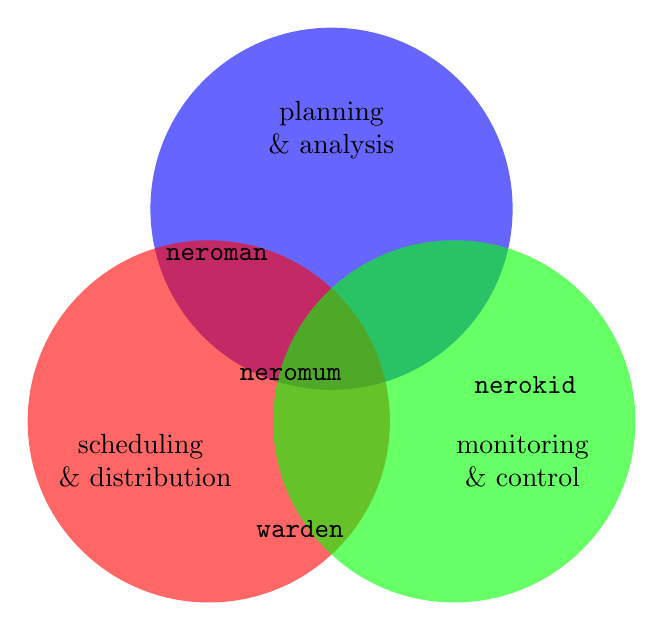
\begin{tikzpicture}[every node/.append style={align=center}]
    \begin{scope}[every path/.append style={opacity=0.6}] % [blend group = soft light]
      \fill[blue]   ( 90:1.8) circle (2.3);
      \fill[red]    (210:1.8) circle (2.3);
      \fill[green]  (330:1.8) circle (2.3);
    \end{scope}
    \node at ( 90:2.8)                {planning \\ \& analysis};
    \node at (210:2.8)                {scheduling \\ \& distribution};
    \node at (330:2.8)                {monitoring \\ \& control};
    \node at (140:1.9)                {\texttt{neroman}};
    \node at (210:0.6)                {\texttt{neromum}};
    \node at (260:2.3)                {\texttt{warden}};
    \node at (350:2.5)                {\texttt{nerokid}};
  \end{tikzpicture}
  \end{figure}
\end{frame}
\begin{frame}{Journey map}
  \begin{figure}
  \tikzset{
    jmi/.append style={align=center,font=\tiny,shape=circle,draw,fill=gray!30,
    minimum size=1.4cm}, jmc/.style={font=\normalsize},
    man/.style={fill=blue!30}, mum/.style={draw=red,thick},
    kid/.style={fill=green!30}, nm/.style={color=blue},
    nj/.style={color=green}, jm/.style={color=red}
  }
  \resizebox{0.8\columnwidth}{!}{
  \begin{tikzpicture}
    \node (00)            [jmi,jmc]          {Research \\ journey};
    \node (01) at (180:4) [jmi]              {Innovate \\ ideas};
    \node (02) at (150:4) [jmi]              {Review \\ literature};
    \node (03) at (120:4) [jmi]              {Write \\ code};
    \node (04) at ( 90:4) [jmi,man]          {Embed \\ analytics};
    \node (05) at ( 60:4) [jmi,man]          {Design \\ tests};
    \node (06) at ( 30:4) [jmi,man,mum]      {Launch \\ tests};
    \node (07) at (  0:4) [jmi,kid,mum]      {Check \\ progress};
    \node (08) at (330:4) [jmi,kid,mum]      {Abort \\ failures};
    \node (09) at (300:4) [jmi,kid,mum]      {Collect \\ results};
    \node (10) at (270:4) [jmi,man]          {Analyse \\ results};
    \node (12) at (225:4) [jmi]              {Publish/drop \\ results};
    \foreach \a/\b in {00/01,01/02,02/03,03/04,04/05,05/06,06/07,07/08,08/09,09/10,10/01,10/12,12/00}
      \draw [->] (\a) edge (\b);
    \node (nm) at ( 30:2) [nm]               {\texttt{neroman}};
    \node (nm) at (  0:2) [jm]               {\texttt{neromum}};
    \node (nj) at (330:2) [nj]               {\texttt{nerokid}};
  \end{tikzpicture}
  }
  \end{figure}
\end{frame}
\begin{frame}{Basic use case}
  \begin{itemize} \scriptsize
  \item \textbf{User}: A computational researcher
  \item \textbf{Goal}: To test how well a new design works with several
    different configuration options and parameter values
  \item \textbf{Preconditions}: SLURM cluster and Neronet setup, code and
    analytics developed and test inputs setup in Neronet compatible manner
  \item \textbf{Basic flow}:
    \begin{enumerate} \tiny
    \item Specify a batch of \Nerokid{}s in the \emph{config YAML}
      with parameters, inputs and other configurations
    \item Dispatch the jobs to the SLURM setup with autogenerated
      \texttt{sbatch} scripts and arguments:
      \texttt{neroman --submit triton 124-186}
    \item Receive and check progress notifications from email    
    \item Monitor the experiment to see near realtime updates of analytics
      variable updates: \texttt{neroman --submit triton 124-186}
    \item Receive final results data and updates. To a log data file.
    \item Analyse, reiterate and/or publish results
    \end{enumerate}
  \item \textbf{Post conditions}: Computational experiments have been
    conducted in a very straightforward, effective and researcher friendly
    fashion
  \end{itemize}
\end{frame}
\section{Components}
\begin{frame}{Components}
  \begin{itemize}
  \item All Nero components are lightweight Python programs run with just the
    researcher's privileges on any modern *nix
  \item SSH is used for communication between \Neroman{} and \Neromum{}s
    (user's existing ssh keys, ssh configs and privileges are used)
  \item Sockets are used between \Neromum{}s and \Nerokid{}s
  \item \Neromum{} communicates with any \Warden{}s using their CLIs
    and/or APIs
  \item The system is ment to be easy to setup, lightweight and the
    usability good for several types of uses.
  \end{itemize}
\end{frame}
\begin{frame}{Communication}
  \begin{figure}
  \tikzset{
    ndom/.style={align=left}
    ncmp/.style={align=center,font=\small,shape=circle,draw,minimum size=3cm},
    ncmp/.style={align=center,font=\small,shape=circle,draw,minimum size=3cm},
    nmum/.style={align=center,font=\small,shape=circle,draw,minimum size=2cm},
    njob/.style={align=center,font=\tiny,shape=circle,draw,fill=green!30},
  }
  \resizebox{0.8\columnwidth}{!}{
    \begin{tikzpicture}
      \draw[dashed] ( 0, 6  ) rectangle (11,11);
      \draw[dashed] ( 0, 0  ) rectangle (11, 5);
      \node (ln) at ( 2,10  ) [ndom]                 {Local network};
      \node (ln) at ( 2, 4  ) [ndom]                 {Cluster network};
      \node (nm) at ( 6, 9  ) [ncmp,fill=blue!30]    {\texttt{neroman}};
      \node (mm) at ( 6, 5.5) [nmum,fill=red!30]     {\texttt{neromum}};
      \node (jm) at ( 8, 2  ) [ncmp,fill=red!30]     {\texttt{warden}};
      \node (j1) at ( 1, 2  ) [njob]                 {\texttt{nerokid}};
      \node (j2) at ( 5, 1  ) [njob]                 {\texttt{nerokid}};
      \node (j3) at (3.8,3) [njob]                 {\texttt{nerokid}};
      \foreach \a/\b in {nm/mm,mm/jm,jm/j1,jm/j2,jm/j3,mm/j1,mm/j2,mm/j3}
        \draw [<->] (\a) edge (\b);
    \end{tikzpicture}
  }
  \end{figure}
\end{frame}
\begin{frame}{\texttt{neroman}}
  % Description of the component its responsibilities, interfaces, and what
  % are the used frameworks and technologies.
  \begin{itemize}
  \item A daemon administered and configured by the researcher herself
  \item Should be run on a system with two way SSH access to the cluster
    gateway or nodes where the \Neromum{}s are deployed
  \item Key functionality
    \begin{itemize}
    \item Facilitate and standardize experiment specification
    \item Batch submit experiment jobs to \Neromum{}s
    \item Send email notifications with progress data
    \item Facilitate monitoring and control of running jobs
    \item Autocollect key job results into a researcher specifiable format
      (f. ex. Excel)
    \item Facilitate experiment analysis and history management
    \item Lightweight and extendable with custom functionality
    \item Configurable via YAML files
    \end{itemize}
  \end{itemize}
\end{frame}
\begin{frame}{\texttt{neromum}}
  % Description of the component its responsibilities, interfaces, and what
  % are the used frameworks and technologies.
  \begin{itemize}
  \item A daemon started and administered by a \Neroman{}.
  \item Should be run on a system with two way SSH access to the \Neroman{}
    and socket access to the nodes where \Nerokid{}s are deployed
  \item Collaborates with standard \Warden{}s.\footnote{SLURM is currently
    used by Triton and CSC. OGE is still used worldwide. Jobman could be
    setup for the CS gpu cluster.}
  \item Key functionality
    \begin{itemize}
    \item Receive and execute commands from \Neroman{}
    \item Communicate with any \Warden{}s by autogenerating job scripts
      (eg. \texttt{sbatch}) and their CLIs and/or APIs.
    \item Collect information from \Nerokid{}s, process and cache them,
      send them to \Neroman{} on request
    \item Transmit commands from \Neroman{} to the \Nerokid{}s
    \end{itemize}
  \end{itemize}
\end{frame}
\begin{frame}{\texttt{nerokid}}
  % Description of the component its responsibilities, interfaces, and what
  % are the used frameworks and technologies.
  \begin{itemize}
  \item A daemon started and administered by a \Neromum{} directly or through
    a \Warden{} on any modern *nix system (typically a cluster node) to start
    and monitor computational jobs
  \item Key functionality
    \begin{itemize}
    \item Send information to \Neroman{} via \Neromum{} as configured
      \begin{itemize}
      \item computing environment information
      \item experiment job progress information read either through an API
      or by parsing output logs and data files (eg. CSV, JSON)
      \end{itemize}
    \item Interact with the \Warden{} as specified (eg. autotermination
      based on poor experiment progress)
    \item Lightweight and extendable with custom functionality
    \item Configurable via YAML files and perhaps a Python API
    \end{itemize}
  \end{itemize}
\end{frame}
% \section{Views}
% \begin{frame}{View 1}
%   An enlightning view.
%   % Read https://leanpub.com/visualising-software-architecture/read
% \end{frame}
% \begin{frame}{View 2}
%   Another enlightning view.
%   % Read https://leanpub.com/visualising-software-architecture/read
% \end{frame}
% \begin{frame}{View 3}
%   Yet another enlightning view.
%   % Read https://leanpub.com/visualising-software-architecture/read
% \end{frame}
\section{Remarks}
\begin{frame}{Remarks}
  \begin{itemize}
  \item A server (\Neroman{}) per user approach is chosen because
    \begin{itemize}
    \item easy minimalist setup (easy to try)
    \item no need for special privileges
    \item fully customizable by the user herself
    \item low resources overhead per setup
    \item total number of users relatively low as well
    \end{itemize}
  \item SSH is used because
    \begin{itemize}
    \item it is an existing standard among target system environments
    \item user's existing SSH keys and configs provide an easy and effective
      way to provide secure networking
    \item no need for network, port routing or privileges adjustments
    \end{itemize}
  \end{itemize}
\end{frame}
\begin{frame}{Remarks}
  \begin{itemize}
  \item Python 3 is used because
    \begin{itemize}
    \item it is already available in most modern *nix systems
    \item it has good support for the known software requirements
    \item it is already popular among computational researchers
    \item many related research libraries use it
      (Scipy, Numpy, Theano, Lasange, Pylearn, Blocks)
    \end{itemize}
  \item Sockets are used because
    \begin{itemize}
    \item they provide fast and efficient realtime communication in tightly
      connected networks
    \item they are lightweight for the cluster filesystem
    \end{itemize}
  \end{itemize}
\end{frame}
% \section{Used languages}
% \begin{frame}{Python 3}
%   Python is the main language to use Lasange, Pylearn2, Theano and Django
% \end{frame}
% \begin{frame}{C++}
%   Main language to use Torch framework.
% \end{frame}
% \begin{frame}{Qt}
%   Optionally can be used to create a user friendly GUI. Can also be used to launch python scripts.
% \end{frame}
% \section{Used libraries}
% \begin{frame}{Django}
%   The framework used to create the web interface for the system.
% \end{frame}
% \begin{frame}{Theano}
%   Main tool to train neural networks, most libraries are built onto this library.
%   % Read https://leanpub.com/visualising-software-architecture/read
% \end{frame}
% \begin{frame}{Torch}
%   Another popular deep leaning framework we plan to support.
% \end{frame}
\end{document}